%%%%%%%%%%%%%%%%%%%%%%%%%%%%% Define Article %%%%%%%%%%%%%%%%%%%%%%%%%%%%%%%%%%
\documentclass{article}
%%%%%%%%%%%%%%%%%%%%%%%%%%%%%%%%%%%%%%%%%%%%%%%%%%%%%%%%%%%%%%%%%%%%%%%%%%%%%%%

%%%%%%%%%%%%%%%%%%%%%%%%%%%%% Using Packages %%%%%%%%%%%%%%%%%%%%%%%%%%%%%%%%%%
\usepackage{geometry}
\usepackage{graphicx}
\usepackage{amssymb}
\usepackage{amsmath}
\usepackage{amsthm}
\usepackage{empheq}
\usepackage{mdframed}
\usepackage{booktabs}
\usepackage{lipsum}
\usepackage{graphicx}
\usepackage{color}
\usepackage{psfrag}
\usepackage{pgfplots}
\usepackage{bm}

%%%%%%%%%%%%%%%%%%%%%%%%%%%%%%%%%%%%%%%%%%%%%%%%%%%%%%%%%%%%%%%%%%%%%%%%%%%%%%%

% Other Settings

%%%%%%%%%%%%%%%%%%%%%%%%%% Page Setting %%%%%%%%%%%%%%%%%%%%%%%%%%%%%%%%%%%%%%%
\geometry{a4paper}

%%%%%%%%%%%%%%%%%%%%%%%%%% Define some useful colors %%%%%%%%%%%%%%%%%%%%%%%%%%
\definecolor{ocre}{RGB}{243,102,25}
\definecolor{mygray}{RGB}{243,243,244}
\definecolor{deepGreen}{RGB}{26,111,0}
\definecolor{shallowGreen}{RGB}{235,255,255}
\definecolor{deepBlue}{RGB}{61,124,222}
\definecolor{shallowBlue}{RGB}{235,249,255}
%%%%%%%%%%%%%%%%%%%%%%%%%%%%%%%%%%%%%%%%%%%%%%%%%%%%%%%%%%%%%%%%%%%%%%%%%%%%%%%

%%%%%%%%%%%%%%%%%%%%%%%%%% Define an orangebox command %%%%%%%%%%%%%%%%%%%%%%%%
\newcommand\orangebox[1]{\fcolorbox{ocre}{mygray}{\hspace{1em}#1\hspace{1em}}}
%%%%%%%%%%%%%%%%%%%%%%%%%%%%%%%%%%%%%%%%%%%%%%%%%%%%%%%%%%%%%%%%%%%%%%%%%%%%%%%

%%%%%%%%%%%%%%%%%%%%%%%%%%%% English Environments %%%%%%%%%%%%%%%%%%%%%%%%%%%%%
\newtheoremstyle{mytheoremstyle}{3pt}{3pt}{\normalfont}{0cm}{\rmfamily\bfseries}{}{1em}{{\color{black}\thmname{#1}~\thmnumber{#2}}\thmnote{\,--\,#3}}
\newtheoremstyle{myproblemstyle}{3pt}{3pt}{\normalfont}{0cm}{\rmfamily\bfseries}{}{1em}{{\color{black}\thmname{#1}~\thmnumber{#2}}\thmnote{\,--\,#3}}
\theoremstyle{mytheoremstyle}
\newmdtheoremenv[linewidth=1pt,backgroundcolor=shallowGreen,linecolor=deepGreen,leftmargin=0pt,innerleftmargin=20pt,innerrightmargin=20pt,]{theorem}{Theorem}[section]
\theoremstyle{mytheoremstyle}
\newmdtheoremenv[linewidth=1pt,backgroundcolor=shallowBlue,linecolor=deepBlue,leftmargin=0pt,innerleftmargin=20pt,innerrightmargin=20pt,]{definition}{Definition}[section]
\theoremstyle{myproblemstyle}
\newmdtheoremenv[linecolor=black,leftmargin=0pt,innerleftmargin=10pt,innerrightmargin=10pt,]{problem}{Problem}[section]
%%%%%%%%%%%%%%%%%%%%%%%%%%%%%%%%%%%%%%%%%%%%%%%%%%%%%%%%%%%%%%%%%%%%%%%%%%%%%%%

%%%%%%%%%%%%%%%%%%%%%%%%%%%%%%% Plotting Settings %%%%%%%%%%%%%%%%%%%%%%%%%%%%%
\usepgfplotslibrary{colorbrewer}
\pgfplotsset{width=8cm,compat=1.9}
%%%%%%%%%%%%%%%%%%%%%%%%%%%%%%%%%%%%%%%%%%%%%%%%%%%%%%%%%%%%%%%%%%%%%%%%%%%%%%%

%%%%%%%%%%%%%%%%%%%%%%%%%%%%%%% Title & Author %%%%%%%%%%%%%%%%%%%%%%%%%%%%%%%%
\title{\textbf{Apuntes de Calculo}}
\author{Matias Leiva Zapata}
%%%%%%%%%%%%%%%%%%%%%%%%%%%%%%%%%%%%%%%%%%%%%%%%%%%%%%%%%%%%%%%%%%%%%%%%%%%%%%%


\begin{document}
\maketitle

\section{Introduccion}
el Calculo es una rama de las matematicas que estudia las variaciones de las cantidades y sus relaciones con otras,
de esta curiosa rama de las matematicas se derivan muchas otras ramas como la Geometria, la Fisica, la Estadistica,
en este recopilatorio de apuntes se intentara abarcar distintos problemas de estas diversas areas.

\section{Problemas:}

% problema numero 2.1

\begin{problem}[Demuestre que:]


\[\int_{0}^{1}(1-x^2)^n dx = \frac{2^{n}{n!}}{(2n+1)!!}\]

\end{problem}




\begin{center}

    \fbox{\parbox[a]{0.985\linewidth}{\textbf{Solucion:}
    %Para poder solucionar esta integral, se debe realizar una sustitucion de variables, 
    %para esto se debe realizar la siguiente sustitucion: u = x^2, de esta forma se obtiene la siguiente integral:


    Para poder solucionar esta integral, se debe realizar una sustitucion de variables
    para esto se debe realizar la siguiente sustitucion: $ u = x^2 $,
    de esta forma se obtiene la siguiente integral:



    \[\int_{0}^{1}{(1-x^2)}^n dx = \frac{1}{2} \int_{0}^{1}{ (1-u)}^n u^{-1/2}du \]


    Luego de esto podemos integrar por partes usando las siguientes variables,
    $ u = (1-x)^n $ y $ v = x^{1/2} $,
    de esta forma se obtiene la siguiente integral:


    \[\frac{1}{2} \int_{0}^{1}{(1-x)}^n x^{-1/2}du =  n\int_{0}^{1}{(1-x)}^{  n-1} x^{1/2}du \]


    inmediatamente podemos volver a integrar por partes usando variables similares,
    \newline
    $u = n{(1-x)}^{n-1} $ y $ v = \frac{2}{3}x^{3/2} $,
    de esta forma se obtiene la siguiente integral:


    \[ n\int_{0}^{1}{(1-x)}^{  n-1} x^{1/2}dx = \frac{2}{3} n(n-1) \int_{0}^{1}{(1-x)}^{n-1}x^{3/2}dx \]


    seguidamente notamos que la integral sigue una clase de recurrencia, la cual podemos escribir como:



    \[I(n) =  2n I(n-1) \]


    iterando nuevamente usando integracion por partes, nos damos cuenta que se obtiene la siguiente integral:


    \[ I(n) = \frac{4}{3}n(n-1)I(n-2) \]



    \[I(n) = \frac{4}{3}\frac{2}{5}n(n-1)(n-2)I(n-3) \]


    \[I(n) = \frac{4}{3}\frac{2}{5}\dots \frac{1}{2n+1} n(n-1)(n-2)\dots (1) I(1) \]



    \[ I(n) =\frac{2^{n}n!} {(2n+1)!!} \]

    }}
\end{center}

\newpage
\fbox{\parbox[a]{0.985\linewidth}{\textbf{Solucion 2:}

        Para poder solucionar esta integral, se integra por partes, haciendo la siguiente sustitucion: $ u = (1-x^2)^n $, y $ v = x $, de esta forma se obtiene la siguiente integral:


        \[\int_{0}^{1}{(1-x^2)}^n dx = x(1-x^2)^{n-1}\Big|_0^1 - n(-2)\int_{0}^{1}{x^2(1-x^2)}^{n-1} dx\]


        \[\int_{0}^{1}{(1-x^2)^n dx} =  2n\int_{0}^{1}x^2(1-x^2)^{n-1}dx\]


        \[\mathcal{I}(n) =  2n\int_{0}^{1}(x^2 -1 + 1){(1-x^2)}^{n-1}dx \]

        \[\mathcal{I}(n) = 2n\mathcal{I}(n) - 2n\mathcal{I}(n-1)\]

        \[\mathcal{I}(n) = \frac{2n}{2n+1}\mathcal{I}(n-1)\]

        \[\mathcal{I}(n) = \frac{2n}{2n+1}\frac{2(n-1)}{2(n-1)+1}\mathcal{I}(n-2)\]

        \[\mathcal{I}(n) = \frac{2^n n!}{(2n+1)!!}\]

    }}
% problema numero 2.2

\newpage

\begin{problem}[Circulos al infinito.]

Suponga que Circulos de igual diametro estan acomodados apretadamente en n filas dentro de un triangulo equilatero.
Si A es el area del triangulo Y $A_n$ es el area total ocupada por las n filas de circulos, demuestre que:

\begin{center}


    $ \displaystyle\lim_{n \to \infty}   \frac{A_n}{A} = \frac{\pi}{2\sqrt{3}}$

    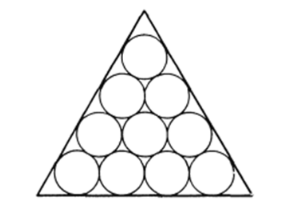
\includegraphics[width=0.23\textwidth,height = 0.2\textwidth]{Triangulo_problema2.2.png}
\end{center}



% Problema Numero 2.3 


\end{problem}


\newpage

\begin{problem}[Sumatoria.]

Determine el intervalo de convergencia de la siguiente sumatoria y calcule la suma.

\begin{center}

    $\displaystyle\sum_{n=0}^{\infty}n^{3}x^n   $
\end{center}


\end{problem}

% Problema Numero 2.4





\newpage

\begin{problem}[Pesadilla del geometra.]

Deduzca la siguiente formula de John Machin:

\begin{center}

    $\displaystyle\ 4\arctan{\frac{1}{5}} - \arctan{\frac{1}{239}} = \frac{\pi}{4}  $
\end{center}


\end{problem}





\end{document}